\documentclass[11pt,letterpaper,spanish]{article}

\usepackage{amsmath,amsthm,amssymb,amsfonts,amsxtra,amstext,anysize,graphicx}

%% Para los usuarios de windows descomentar esta linea y utilizar acentos normalmente.
\usepackage[utf8]{inputenc}
\usepackage[spanish]{babel}
\usepackage{mathrsfs}
\usepackage{fullpage}
\usepackage{verbatim}
\usepackage{graphicx}
\usepackage{subfigure}
\usepackage{wrapfig}
\usepackage{esint}
\usepackage{epsfig}
\usepackage{epstopdf}
\usepackage{multirow}
\usepackage{caption}
\usepackage{hyperref}
\usepackage{float}
\usepackage{color}
\usepackage{pdfpages}% Se utiliza para poder
%\newcommand{\parrafo}[1]{\paragraph{#1}\mbox{}\\}


%% LaTeX will automatically break titles if they run longer than
%% one line. However, you may use \\ to force a line break if
%% you desire.
\usepackage{color}
\definecolor{gray97}{gray}{.97}
\definecolor{gray75}{gray}{.75}
\definecolor{gray45}{gray}{.45}
\usepackage{listings}
\lstset{ frame=Ltb,
framerule=0pt,
aboveskip=0.5cm,
framextopmargin=3pt,
framexbottommargin=3pt,
framexleftmargin=0.4cm,
framesep=0pt,
rulesep=.4pt,
backgroundcolor=\color{gray97},
rulesepcolor=\color{black},
%
stringstyle=\ttfamily,
showstringspaces = false,
basicstyle=\small\ttfamily,
commentstyle=\color{gray45},
keywordstyle=\bfseries ,
%
numbers= none,
numbersep=15pt,
numberstyle=\tiny ,
numberfirstline = false,
breaklines=true,
}

% minimizar fragmentado de listados
\lstnewenvironment{listing}[1][]
{\lstset{#1}\pagebreak[0]}{\pagebreak[0]}

\lstdefinestyle{consola}
{
basicstyle=\scriptsize\bf\ttfamily,
backgroundcolor=\color{gray75},
}

\lstdefinestyle{C}
{language=C,
}




\begin{document} %%Comienza el documento 
\renewcommand{\tablename}{Tabla}

  
\epsfig{file= figuras/logonitido, width= 2.3 cm} %% Agrega una imagen
    \begin{tabular}{l}%% tabular va con una "l" no con un uno
    Pontificia Universidad Cat\'olica de Chile\\
    Escuela de Ingenier\'ia\\
    Departamento de Ingenier\'ia El\'ectrica\\
  \vspace{1.9 cm}\mbox{}
    \end{tabular}
    \bigskip
 
\begin{center}
\huge{Manual para la creación de placas PCB\\ multi-capa con el software Eagle.}\\
%\Large{\textbf{}}\\
%\normalsize{3- Sesiones}
\vspace{0.5 cm}
\hrule
\vspace{0.1 cm}
\hrule
\end{center}
\vspace{0.2 cm}
\section{Introducción}
\par 
 Esta guía es una recopilación de la información existente en internet y variadas fuentes. Tiene como objetivo entregar el conocimiento necesario para el diseño de placas multi-capas en el software Eagle.  Esta guía asume que el lector esta familiarizado con el software. Finalmente se incluye una serie de consejos recopilados útiles al momento de diseñar una placa.
\section{Configuración inicial}
Lo primero que debemos hacer es indicarle a Eagle que la placa en la que trabajaremos es multi-capa\footnote{Esto solo es posible para las versiones licenciadas de Eagle.}. En la ventana de board, por defecto solo existen dos capas: la capa de top (asignada como layer 1) y la capa de bottom (asignada como layer 16). Para habilitar tantas capas como necesitemos debemos ir a \verb+Edit/Design rules+. En la ventana de reglas de diseño seleccionamos la pestaña \verb+Layer+. En este punto debemos familiarizarnos con el concepto de VIA.

\subsection{VIA}
VIA es la sigla en ingles para Vertical Interconnect Access. Son agujeros en las placas que permiten conectar las señales entre capas. Las VIA pueden ser de tres tipos:
\begin{center}
\begin{description}
\item[Through hole:] Es el tipo de VIA más común, y constituye una conexión entre todas las placas desde la inicial (denominada  top), hasta la placa final (bottom).
\item[Blind:] Este tipo de VIA representa una conexión entre capas internas de la placa. Por ejemplo, si estamos trabajando con una placa de 5 capas, las  VIA del tipo Blind son todas aquellas que conecten cualquier capa desde la capa 2 a la capa 4.
\item[Buried:] Finalmente, este tipo de VIA permite la conexión entre una capa interna de la placa y alguna de las dos capas extremas (top o bottom).
\end{description}
\end{center}

\begin{figure}[!H]
\begin{center}
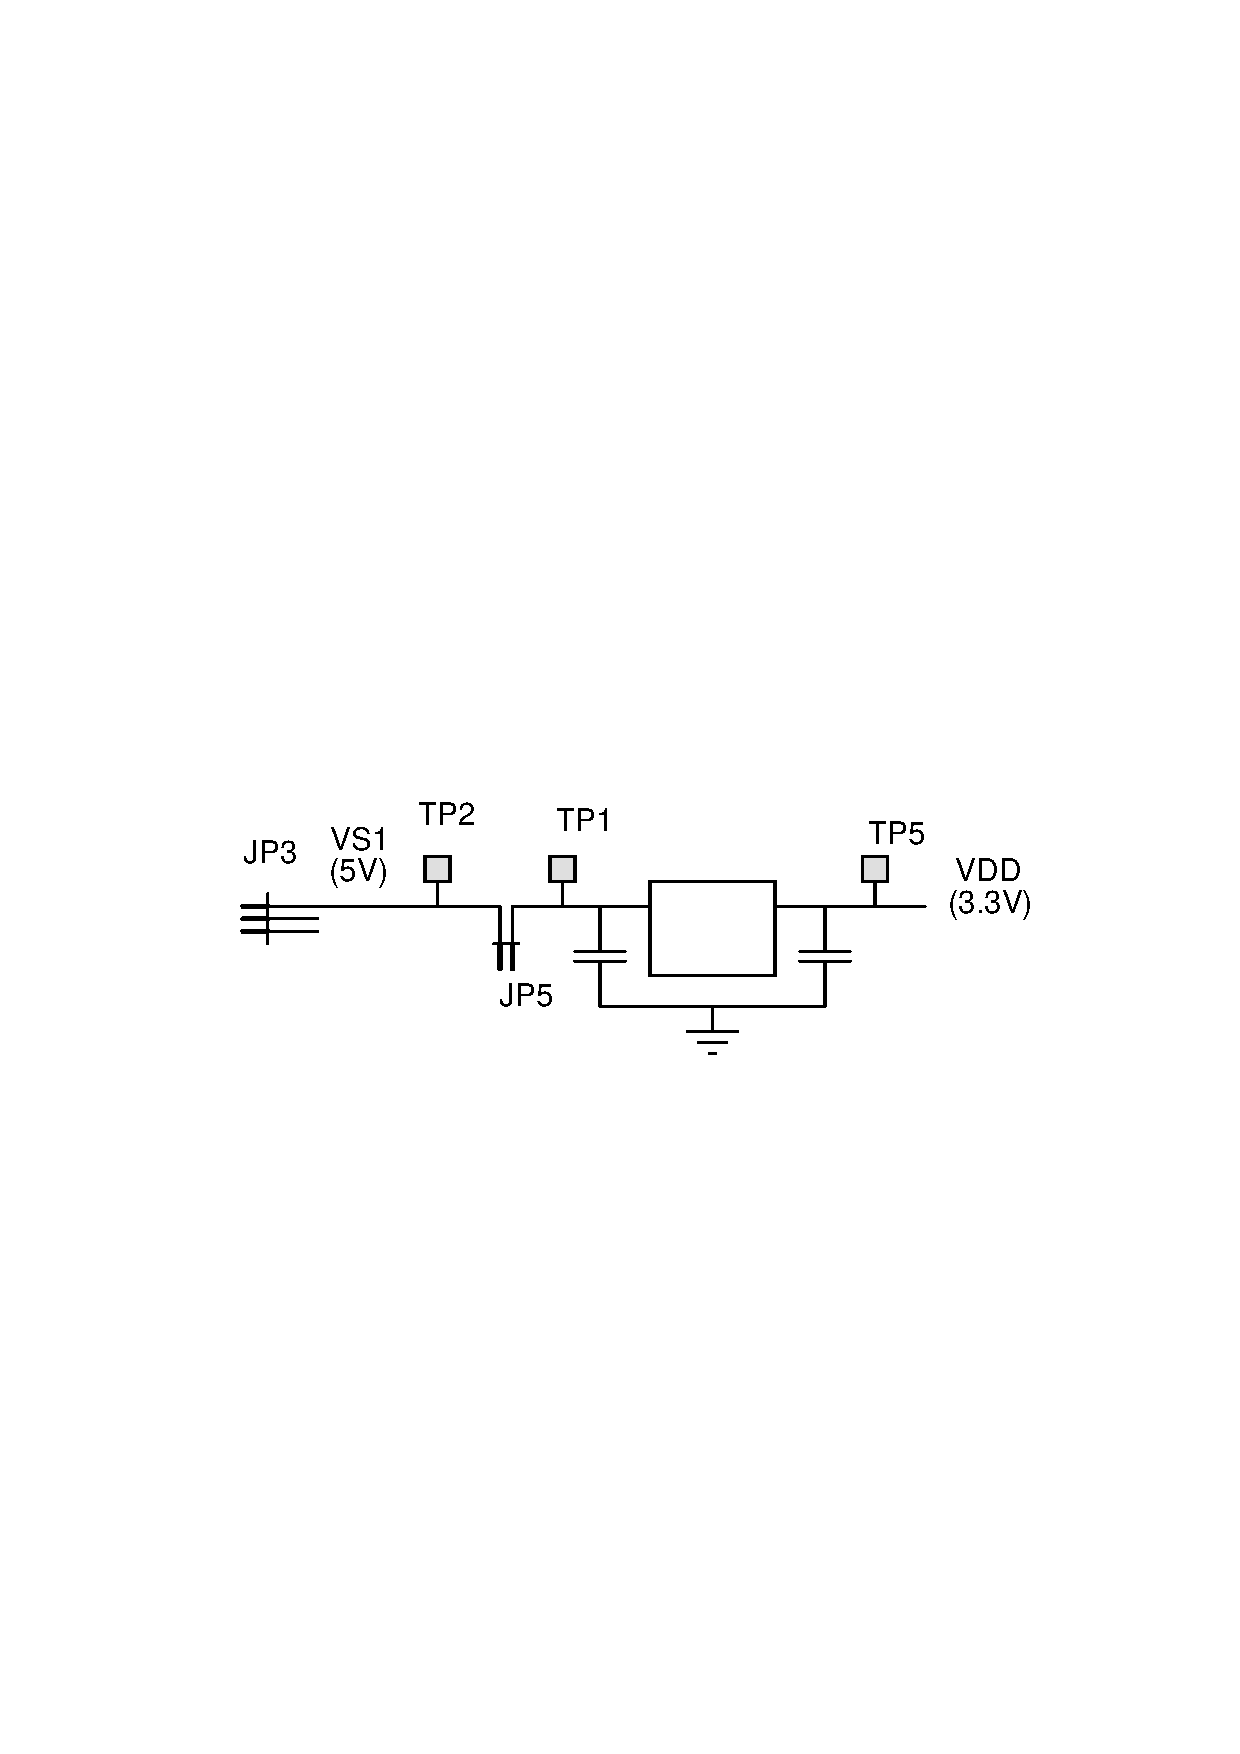
\includegraphics[scale=0.5]{figuras/1.JPG}
\end{center}
\caption{1.Trhoug hole VIA, 2.Blind VIA, 3.Burried VIA}
\end{figure}

El paso siguiente es indicar en la sección \verb+Setup+ cuales serán las características de nuestra placa y como serán sus conexiones con el resto de la placa\footnote{Es importante tener en cuenta que tipo de conexiones son permitidas por el fabricante, ya que no siempre están todas disponibles y poseen distintos costos asociados.}. Para esto Eagle cuenta con una notación especifica en donde las conexiones Buried y Through se implementan con el formato \verb+(a*b)+. Las conexiones Blind se indican con el formato \verb+[t:..:b]+ donde t representa la capa de inicio y b la final.

Asi por ejemplo si queremos una placa de 4 capas con una conexión del tipo Through entre todas las capas y conexiones del tipo Blind entre las dos superiores y las dos inferiores debemos anotar lo siguiente: 

\begin{verbatim}
Setup: [2:(1*2*3*16):3]
\end{verbatim}

El resultado se puede apreciar en la figura \ref{setup2}.

\begin{figure}[!h]
\begin{center}
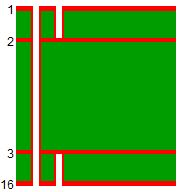
\includegraphics[scale=0.5]{figuras/2.JPG}
\end{center}
\caption{\label{setup2} Configuración de una placa de 4 capas con conexiones tipo through y blind.}
\end{figure}

Una vez configurado el tipo de placa en el que trabajaremos podemos comenzar a agregar los componentes.

\section{Creación de un componente nuevo}
En Eagle existe una extensa cantidad de librerías disponibles, en donde podemos encontrar los componentes que necesitamos. El caso de interés es cuando nuestro componente no se encuentra en ninguna de las librerías de Eagle. En tal caso, lo primero que debemos realizar es actualizar las librerías con las que contamos, esto lo podemos realizar desde la página del proveedor, en \url{http://www.cadsoftusa.com/downloads/libraries}. 
Si aun no encontramos nuestro componente en un librería existente debemos crearlo por nuestra cuenta. Para esto, una buena practica es crear nuestra propia librería de trabajo.
 Debemos ir al panel de control de Eagle seleccionamos la opción \verb+File/New/Library+.\\ Cada nuevo componente que crearemos se compone de 3 partes:
\begin{enumerate}
\item Package
\item Symbol
\item Device
\end{enumerate}
\subsection{Package\label{package}}
En esta sección se debe crear el Package del componente o empaquetado. Para esto debemos recurrir al datasheet del componente y ver que tecnología utilizan. En la ventana de librería vamos a \verb+Library/Package+ o utilizamos el atajo de la barra de herramientas. En la sección \verb+New+ agregamos el nombre del componente y aceptamos. 
En la nueva ventana se agregan nuevas opciones a nuestra barra de herramientas\footnote{Para más detalle sobre las herramientas recomendamos recurrir al help de Eagle, o escribimos en la barra de comando help comando deseado}, las cuales nos permitirán dibujar el layout que deseamos. 
\begin{description}
\item[Observación:] Es importante mencionar que pese a que muchos componentes no poseen su modelo en las librerías de Eagle, si existe una gran cantidad de empaquetados disponibles los cuales pueden ahorrarnos trabajo al momento de crear un nuevo modelo. Para esto recomendamos abrir la librería ref-packages.lbr en donde podremos encontrar muchos empaquetados estándar los cuales podemos copiar y pegar en nuestra librería.
\end{description}
Como ejemplo veamos el componente OP282 el cual es un amplificador operacional cuyo datasheet esta disponible en el siguiente \href{http://www.analog.com/media/en/technical-documentation/data-sheets/OP282_482.pdf}{link}. En la pagina 14 del documento podemos encontrar la información del empaquetado.

\begin{figure}[!h]
\begin{center}
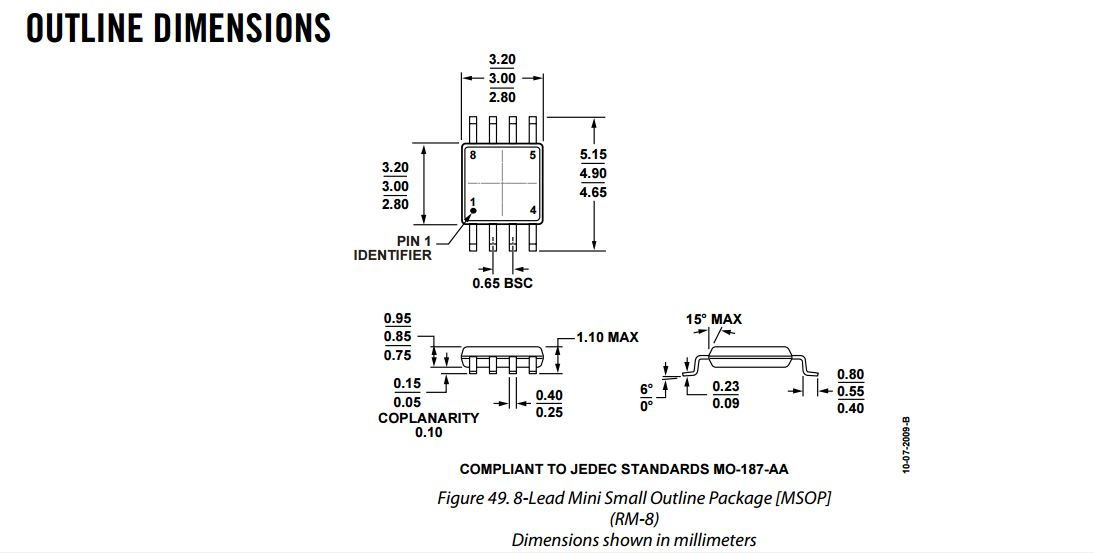
\includegraphics[scale=0.4]{figuras/3.JPG}
\end{center}
\caption{Package entregado por el fabricante del IC op282}
\end{figure}


Utilizando estos datos podemos replicar nuestra propia versión del empaquetado.

\begin{figure}[!h]
\begin{center}

\includegraphics[scale=0.4]{figuras/4.JPG}
\end{center}
\caption{Modelo implementado para el empaquetado del IC op282}
\end{figure}


En el modelo hemos agregado dos textos para agregarle atributos de nombre y valor al integrado, estos textos deben ir en las capas de \verb+tNames+ y \verb+tValue+ respectivamente.


\subsection{Symbol}
Una vez creado el empaquetado que usaremos debemos crear un símbolo que represente a nuestro componente en el esquemático de nuestra placa. Para esto vamos a \verb+Library/Symbol+ o utilizamos el atajo en la barra de herramientas superior y creamos nuestro nuevo símbolo. Una vez en la ventana de símbolos, cambiaran nuevamente las opciones de la barra de herramientas de la izquierda. La idea es crear un símbolo lo mas parecido al que se nos entrega en el datasheet incluyendo los respectivos nombres de cada uno de los pines del componente. Para el integrado op282 podemos encontrar su símbolo en la pagina 1 del datasheet entregado en  \ref{package}.



\begin{figure}[!h]
\begin{center}
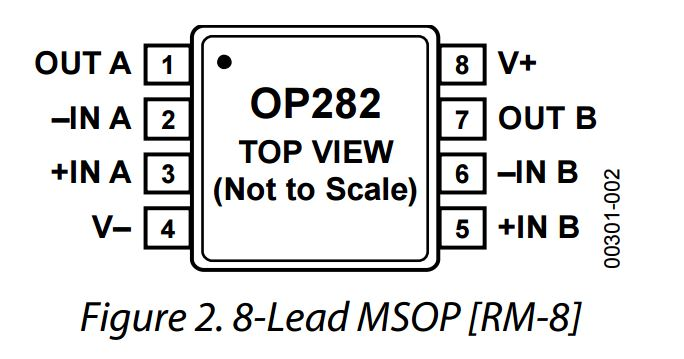
\includegraphics[scale=0.4]{figuras/5.JPG}
\end{center}
\caption{Símbolo entregado por el fabricante del IC op282}
\end{figure}

Procedemos a replicarlo obteniendo un modelo personalizado, al cual le hemos agregado los nombres respectivos de cada pin, junto con el nombre del componente.


\begin{figure}[!h]
\begin{center}
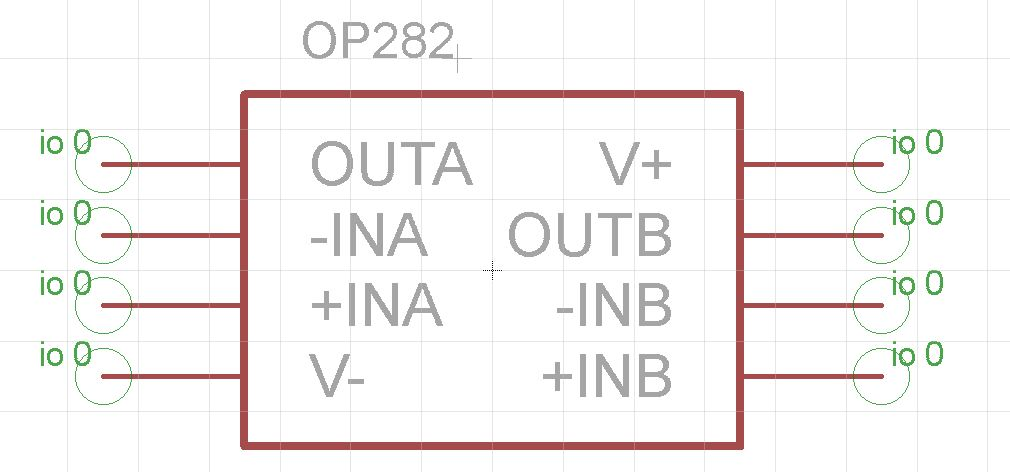
\includegraphics[scale=0.3]{figuras/6.JPG}
\end{center}
\caption{Modelo implementado para el símbolo del IC op282}
\end{figure}

\subsection{Device}
Finalmente el último paso es crear un componente en Eagle el cual cuenta con dos atributos que son un Package y un Symbol. Para esto nos vamos a \verb+Library/Device+ o utilizamos el atajo de la barra de tareas superior y creamos el nuevo device. 
 Utilizamos la herramienta \verb+Add+ o \verb+Edit/Add+ para agregar un nuevo símbolo y seleccionamos el símbolo previamente creado. Posteriormente en la opción \verb+New+ de la sección derecha agregamos el empaquetado previamente creado. El ultimo paso consiste en realizar la conexión entre el símbolo y el modelo del empaquetado lo cual implementamos por medio de la opción \verb+Connect+ y seleccionamos uno a uno como deben ir conectados los pines. También podemos elegir el tipo de prefijo que tendrá nuestro nuevo componente, en la opción \verb+Prefix+.
\begin{description}
\item[Observación] Es recomendable agregar descripciones para nuestro componente creado, ya que esto agrega etiquetas que permiten mejorar la búsqueda del componente o ayudan a una persona externa de que componente se trata.
\end{description} 
 
\section{Componentes con arreglo de pines y uso de scripts en eagle}
	\subsection{Scripts en Eagle}
		\subsubsection{Lista de comandos}
	\subsection{Ejemplo práctico}
\section{Consejos de diseño} 
\end{document}
